\chapter{Introduction} \label{sec:introduction}
\epigraphhead[30]{\epigraph{%
\textit{"A planet is the cradle of mind, but one cannot live in a cradle forever."}}%
{\textsc{Konstantin E. Tsiolkovsky (1857 - 1935)}}%
}

\section{The conquest of space} \label{sec:conquest}

Since in 1609 German mathematician and astronomer Johannes Kepler published his book \textit{Astronomia nova}, containing the most famous of all transcendental equations, the motion of the celestial bodies has attracted the attention of the greatest minds in human history, even sparkling entire new fields in mathematics \cite{battin1999introduction}. It is easy to imagine that if even Kepler's equation, the one that captures the essence of the two-body problem in its most restricted form, already has this mathematical intricacy, any further development will carry away similar or greater complexity.

\begin{figure}[h]
\[M = E - e \sin{E}\]
\caption{The Kepler equation.}
\end{figure}

Almost three centuries later, in 1903, Russian rocket scientist Konstantin E. Tsiolkovsky first explained in his article \textit{Exploration of Outer Space by Means of Rocket Devices} precise conditions for artificial objects to reach the orbit of the Earth, making a huge leap from the mere observation of the celestial bodies and the science fiction stories that had inspired him to the real possibility of going to space. Quoting \cite{siddiqi2000challenge}:

\begin{displayquote}
In his most revolutionary idea, he proposed that humans could hope to fly to very high altitudes and ultimately into outer space only by using liquid-propellant rockets. One of his most  important conclusions was that a rocket would be capable of carrying up a cargo of any size, and develop any speed desired,  as long as the rocket was sufficiently large and the ratio of the mass of the propellant to the mass of the entire rocket was  large enough -- a relationship that is known as the Tsiolkovsky Equation.
\end{displayquote}

% Regarding Saxon genitive and equation names
% http://english.stackexchange.com/a/301270/20057

\begin{figure}[h]
\[\Delta v = v_e \ln \frac{m_0}{m_f}\]
\caption{The Tsiolkovsky equation.}
\end{figure}

If we define the term Astrodynamics as the branch of Mechanics that studies practical problems concerning the motion of rockets and other artificial objects through space, Tsiolkovsky's contribution might well be considered its starting point, and many others ensued before they could be tested in practice during the second half of the 20th century. In 1919 Yuri V. Kondratyuk conceived the gravitational slingshot or flyby to accelerate a spacecraft through interplanetary flight and suggested a mission profile for a Lunar landing \cite{siddiqi2000challenge}, in 1925 Walter Hohmann conjectured that the minimum-fuel transfer between two coplanar circular orbits consists of two tangent impulses along the line of apses (although this result was not proved until almost forty years later in \cite{lawden1963optimal}) and in 1926 Hermann J. Oberth observed that the velocity gain of an impulsive maneuver is higher when the kinetic energy is maximum (nowadays known as the Oberth effect). The severe limitations in weight and available energy for such kind of travels were already apparent for these pioneers, who were, in some way, anticipating the need to optimize on board fuel consumption.

At the same time, important practical advances were being made in the field of rocketry. In 1920 Robert H. Goddard published in his article \textit{A Method of Reaching Extreme Altitudes} several ideas and experimental results regarding the study of rockets, in particular that the exhaust speed of their combustion gases could be greatly increased by using convergent-divergent or De Laval nozzles, and in 1926 he launched the world's first liquid-fueled rocket, which reached an altitude of 12 meters, lasted 2 seconds and averaged about 100 kilometers per hour. After this remarkable event, amateur rocket societies started to form in America and Europe and bigger and more sophisticated rockets were built and launched in the following years.

To this day, chemical propulsion (whether using liquid fuel as pioneered by Goddard and later used by the Saturn V or solid fuel as already used by the Chinese in the 13th century) continues to be the only way to escape the gravitational well of the Earth. What is not so well known is that many of the people involved in the early development of astrodynamics and astronautics in the 20th century shared a common interest in an alternative method: electric propulsion. Goddard had already reflected on the use of "electrons moving with the velocity of light" as a method of propulsion as early as 1906, and Tsiolkovski wrote in 1911 about the use of electricity "to produce a large velocity for the particles ejected from a rocket device" \cite{choueiri2004history}. Oberth even envisioned electric propulsion as a real possibility for attitude control in his 1929 book \textit{Ways to Spaceflight} and already predicted its mass saving capabilities.

Despite all this enthusiasm, however, there were far too many obstacles at the time to make it a reality: first of all, the understanding of atomic physics was still in its infancy, with the nature of the electrons still unclear and the discovery of the proton not happening until 1920, hindering rigorous studies. Besides, electric propulsion was definitely not useful to attain orbital velocity, and on the other hand it requires a much more complex mathematical analysis (we will expand on these aspects in \ref{sec:propulsion}). For the following fifteen years after the publication of Oberth's book all the focus shifted away from electrical propulsion, until the tremendous advances regarding the production of intense ion currents during the forties brought back the debate about its feasibility \cite{choueiri2004history}.

Electric spacecraft propulsion was not the only idea that appeared those years that fell dormant because it was well ahead of its time. In 1925, twenty five years after Pyotr N. Lebedev demonstrated the pressure of light, Friedrich A. Zander published a technical paper titled \textit{Problems of flight by jet propulsion: interplanetary flights} where he discussed several challenges associated with space travel, including re-entry into the Earth atmosphere, and first analyzed with great detail the use of radiation pressure as a mean of propulsion, an idea suggested years earlier by Tsiolkovski. Zander proposed the use of extremely thin aluminum mirrors and computed the required surface and admissible stresses, laying the first bricks of beam-powered propulsion. The first formal technology and design effort for a solar sail did not begin until  1976 and to this day there are no flight proven solutions.

In 1950 George F. Forbes presented the element that was missing for a complete mathematical analysis, the study of low-thrust trajectories, by showing for the first time that in some cases they were more efficient than the high-thrust counterparts in his Masters thesis \textit{The trajectory of a powered rocket in space}. This, and the contribution of Lyman S. Spitzer, who in his 1952 paper \textit{Interplanetary Travel Between Satellite Orbits} suggested that for an ion propulsion system to be technically useful, an acceleration of three centimeters per square second would be enough ("sufficient to attain a velocity of $15~\text{km/sec}$ in two months" \cite{spitzer1952interplanetary}), provided the building blocks for the electrical propulsion to have the attention it deserved.

Finally, the decade of the sixties served as the definitive \textit{tour de force} of chemical propulsion, which powered the rockets used during the space race that started in 1957 with the launch of Sputnik I by the Soviet Union and that culminated with in 1969 with the first manned landing on the Moon by the United States of America. In the meanwhile, in 1964 the first mission to demonstrate the use in orbit of an ion thruster, SERT-1, was launched, whereas a milestone comparable in importance arrived as late as 1998 with the mission Deep Space 1. With these achievements, the early ideas of the visionaries of the beginning of the century were finally proven real and humanity was in the position of using these technologies to "leave the cradle".

\section{Chemical versus electric propulsion} \label{sec:propulsion}

After the historical perspective given in \ref{sec:conquest} we dedicate the following sections to introduce some important theoretical concepts, with the objective of justifying the importance of low-thrust orbit analysis within the context of orbit optimization and the pursuit of analytical solutions in this area. We start with the distinction of chemical versus electric propulsion and the main similarities and differences between them -- this does not intend to be an in-depth description of the subsystems and technologies that are involved, but rather an overview of their most essential aspects and how do they affect their performance and use cases (for such in-depth analysis we direct the readers to well known references in the subject such as \cite{sutton2016rocket}). In \ref{sec:methodstable} a thorough list of spacecraft propulsion methods has been included for reference.

Except for very small satellites, nearly all space missions require on-board propulsion systems, which have a major impact on spacecraft mass \cite{curran1993nasa}. Some sources estimate that the current cost of sending one kilo of payload into low Earth orbit lies around 20~000~€, and therefore any effort to decrease the launch mass of the spacecraft leads to significant savings \cite{choueiri2009new}.

We can define propulsion in a broad sense as the act of changing the motion of a body \cite{sutton2016rocket}. Spacecraft propulsion methods can be classified according to the energy source that is used to produce thrust, which can be chemical, nuclear or electric.

\textbf{Chemical propulsion} uses the chemical potential stored in the propellants, usually of reducing (fuel) and oxidizing nature, that is released in a high-pressure combustion reaction between the two. The reaction produces a flow of hot gases (between 2500 and 4100~\celsius) that can be accelerated in a convergent-divergent (or De Laval) nozzle to achieve supersonic velocities (1800 to 4300 m/s). In this case, therefore, the power source and the propellants are the same elements. Chemical propulsion systems can be themselves subdivided according to the state of the propellants: \textit{solid propellant rocket motors} use a solid material that contains all the chemical elements that are needed for complete burning, whereas \textit{liquid propellant rocket engines} use liquid propellants that are fed under pressure from separate tanks into a thrust chamber, where they react.

\textbf{Electric propulsion} comprises a family of systems that use an electric power source which is physically separate from the mechanism that produces the thrust itself. In \textit{electro-thermal propulsion} the propellant is heated by heated resistors or electric arcs and then expanded to supersonic velocity as it is done in chemical propulsion systems. On the other hand, \textit{ion and plasma drives} use electric and magnetic fields to accelerate ions or highly ionized plasmas, therefore not applying thermodynamic expansion to the propellant.

\textbf{Beam-powered propulsion} or directed energy propulsion refers to a broad family of methods, some of them experimental or speculative, that use an external power source to propel the spacecraft. Some of them concentrate beamed energy to heat a stored propellant, such as solar thermal rockets, while others use passive devices that take advantage of the radiation pressure, such as solar or laser-based sails.

Lastly, \textbf{nuclear propulsion} is a proposed spacecraft propulsion technology that delivers heat to a working fluid by means of a nuclear reaction, either by atomic fission or fusion. While they would be extremely useful for shortening interplanetary travel time and the first are at least feasible with today's technology, to date no nuclear thermal rocket has flown and they present too many technological and environmental problems, so we won't discuss more about them.

To this day, no optimal spacecraft propulsion method exists and when designing an space mission one or more of them must be chosen according to the desired requirements and the available technology. Figure \ref{fig:propulsionchart} displays a graphical summary of performance characteristics of several spacecraft propulsion methods according to their energy source. As mentioned before, the only method that has enough power to escape the gravitational field of the Earth is chemical propulsion, whether in the form of solid rockets or liquid engines: the rest of the methods provide an acceleration (or, equivalently, thrust) that is orders of magnitude below and that does not reach the required thrust-to-drag ratio to lift the spacecraft to the atmosphere.

\begin{figure}
\centering
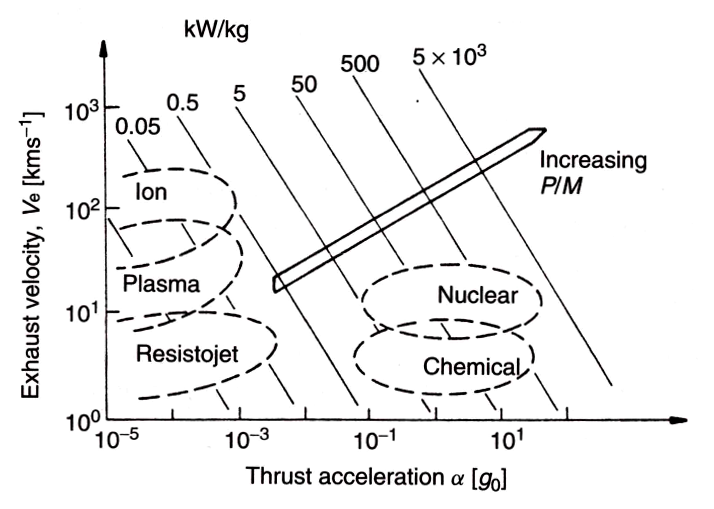
\includegraphics[width=1.0\textwidth]{figures/propulsion-diagram.png}
\caption{Performance characteristics of spacecraft propulsion methods according to energy source.}
\label{fig:propulsionchart}
\end{figure}

However, chemical propulsion is not without limitations. If we recover the Tsiolkovski equation

\begin{equation}
\Delta v = v_e \ln \frac{m_0}{m_f}
\end{equation}

we notice that the obtained increment in velocity $\Delta v$ is directly proportional to the \textit{effective exhaust velocity} $v_e$ and that increases with the \textit{mass fraction} $m_0 / m_f$. Effective exhaust velocity can be also written as

\[
% * <dmorante@ing.uc3m.es> 2017-02-28T20:08:33.734Z:
%
% ^.
v_e = I_{sp} g_0 = \frac{T}{\dot{m}}
\]

where $I_{sp}$ is the specific impulse, $g_0$ is the standard gravity, $T$ is the exerted thrust and $\dot{m}$ is the mass flow rate. Therefore, $v_e$ is a measure of the \textit{efficiency} of the propulsion system. If our effective exhaust velocity (or, equivalently, specific impulse) is low, we will need a higher mass fraction to gain the required velocity increment. Notice that this equation is ideal and does not take into account loses due to atmospheric drag or the gravitational forces.

While the maximum thrust achievable with chemical propulsion is more than $10^6$ newton, the specific impulse using current technology is in the range of 250 to 500 seconds approximately. This is a comparatively low value for the efficiency and creates the need of carrying high amounts of propellant mass, both for expendable rockets that raise the payload into orbit and also for attitude control and orbit maintenance systems for the operation of the spacecraft \cite{curran1993nasa}.

Fortunately, the specific impulse for ion thrusters and plasma drives can be one or two orders of magnitude higher, therefore leading to much lower propellant mass requirements. However, although these systems are more efficient in terms of the consumed mass for a given trajectory, due to the limitation of electrical power on board the spacecraft the available thrust is significantly lower than chemical rockets. As a result, low-thrust systems in general and electric propulsion systems in particular must be used during long periods of time that can range between weeks and months.

This sole fact renders the mathematical treatment of low-thrust trajectories much more complicated: on the one hand they cannot be treated as ballistic arcs anymore since there will be a permanent force acting on the spacecraft in addition of the gravitational field, and on the other hand there will be an infinite number of possible trajectories between two points and fixed times \cite{woodcock2002benefits}. In the following sections we analyze the consequences of these two facts.

\section{The perturbed two-body problem}

The equation of the perturbed relative motion of two bodies is \cite{battin1999introduction}

\begin{equation}
\deriv[2]{\vec{r}}{t} + \frac{\mu}{r^3} \vec{r} = \vec{a}_d
\label{eq:twobody}
\end{equation}

% {Battin 84, 94, 10.3}

where $\vec{r}$ is the position vector of one body with respect to another, in our case the spacecraft with respect to its attractor, and $\vec{a}_d$ is the non-Keplerian or perturbation acceleration. This equation arises when analyzing the n-body problem, in which case the perturbation acceleration is due to the gravitational attraction of the other $n - 2$ bodies, but $\vec{a}_d$ can be more general and include the action of a low-thrust device. This action can be controlled in the case of electric propulsion systems or be subject to external factors in the case of beam-powered propulsion systems such as the radiation pressure from the Sun.
% * <dmorante@ing.uc3m.es> 2017-02-28T20:31:33.757Z:
% 
% >  perturbation acceleration
% perturbing acceleration
% 
% ^ <dmorante@ing.uc3m.es> 2017-02-28T20:35:54.631Z.
% * <dmorante@ing.uc3m.es> 2017-02-28T19:48:59.231Z:
% 
% > vector position
% position vector
% 
% ^ <juanlu001@gmail.com> 2017-02-28T21:54:11.552Z.

The most straightforward method for determining the position $\vec{r}(t)$ and velocity $\vec{v}(t)$ in the case of a nonzero perturbing acceleration is a direct numerical integration of \ref{eq:twobody} in rectangular coordinates, known as Cowell's method \cite{battin1999introduction}. However, this equation becomes singular when the distance between the two bodies approaches zero, is nonlinear and its solution is unstable, so a number of regularizations and transformations have been proposed in the literature \cite{bau2013new}.
% * <dmorante@ing.uc3m.es> 2017-02-28T20:10:48.158Z:
% 
% > the two bodies
% Al principio empiezas hablando de 'target mass' y de 'attractor'  luego pasas directamente  a hablar de 'bodies'. Trata de conectarlo alguna manera o modificarlo
% 
% ^ <juanlu001@gmail.com> 2017-02-28T22:15:04.583Z:
%
% reescrita la primera frase
%
% ^ <juanlu001@gmail.com> 2017-02-28T22:15:07.391Z.
% * <dmorante@ing.uc3m.es> 2017-02-28T20:09:20.531Z:
% 
% > However, this equation is nonlinear, becomes singular when the distance between the two bodies becomes zero and its solution is unstable, so a number of regularizations and transformations have been proposed in the literature
% However, this equation is singular when... (o reformular de alguna otra manera)
% 
% ^ <juanlu001@gmail.com> 2017-02-28T21:55:31.446Z.
% * <dmorante@ing.uc3m.es> 2017-02-28T20:03:59.461Z:
% 
% >  if
% is
% 
% ^ <juanlu001@gmail.com> 2017-02-28T21:55:57.066Z.
% * <dmorante@ing.uc3m.es> 2017-02-28T19:58:59.921Z:
% 
% >  $\vec{r}(t)$
% $\vec{v}(t)$
% 
% ^ <juanlu001@gmail.com> 2017-02-28T21:56:55.255Z.

Another approach to integrate the equations of motion is to use a set of orbital elements as dependent variables and then apply variational techniques. This technique, called \textit{variation of parameters}, assumes that we can use the solution of the unperturbed system to represent the complete solution \cite{vallado2001fundamentals}. The advantage is that most orbital elements stay constant for the case of pure Keplerian motion, and depending on the nature of the perturbing forces, the effects on the orbit can be circumscribed to a small subset of orbital elements. Furthermore, we can easily separate the short period, long period and secular effects on each of those elements. Two forms of variational equations exist: the Lagrangian form assumes the perturbation function can be derived from a potential, and the Gaussian form removes this constraint \cite{battin1999introduction}. The former is useful when analyzing conservative perturbations, like the effects of the non-spherical shape of the Earth, whereas the latter is more general and works for arbitrary perturbation accelerations.
% * <dmorante@ing.uc3m.es> 2017-02-28T20:14:05.058Z:
% 
% > exist
% aquí añadiría referencia
% 
% ^ <juanlu001@gmail.com> 2017-02-28T21:58:33.088Z.
% * <dmorante@ing.uc3m.es> 2017-02-28T20:13:37.464Z:
% 
% Aquí añadiría referencia
% 
% ^ <dmorante@ing.uc3m.es> 2017-02-28T20:14:01.833Z.

There are many forms of the Gauss planetary equations, depending on the element set in use and the reference frame chosen for projecting the perturbation acceleration components. We reproduce here the form derived by \cite{battin1999introduction}, which uses classical orbital elements $(a, e, i, \Omega, \omega, M)$ and polar coordinates $(f_r, f_{\ta}, f_h)$:
% * <dmorante@ing.uc3m.es> 2017-02-28T20:22:40.780Z:
% 
% > $(f_r, f_{\ta}, f_h)$
% Convendría aclarar cuál es el sistema de coordenadas polares que se utiliza (porque podría ser cualquiera)
% 
% ^ <dmorante@ing.uc3m.es> 2017-02-28T20:26:13.404Z.
% * <dmorante@ing.uc3m.es> 2017-02-28T20:19:26.012Z:
% 
% >  perturbation acceleration
% perturbing acceleration
% 
% ^ <dmorante@ing.uc3m.es> 2017-02-28T20:35:46.253Z.
% * <dmorante@ing.uc3m.es> 2017-02-28T20:14:42.716Z:
% 
% > element set
% set of elements
% 
% ^ <juanlu001@gmail.com> 2017-02-28T21:59:58.184Z:
%
% Lo he visto así escrito en muchos sitios
%
% ^ <juanlu001@gmail.com> 2017-02-28T22:00:01.877Z.

\begin{align}
\deriv{a}{t} & = \frac{2 a^2}{h} \left( e \sin{\ta} f_r + \frac{p}{r} f_{\ta} \right) \\
\deriv{e}{t} & = \frac{1}{h} \left( p \sin{\ta} f_r + \left( \left( p + r \right) \cos{\ta} + r e \right) f_{\theta} \right) \\
\deriv{i}{t} & = \frac{r \cos{\arglat}}{h} f_h \\
\deriv{\Omega}{t} & = \frac{r \sin{\arglat}}{h \sin{i}} f_h \\
\deriv{\omega}{t} & = \frac{1}{he} \left( -p \cos{\ta} f_r + \left( p + r \right) \sin{\ta} f_{\theta} \right) - \frac{r \sin{\arglat} \cos{i}}{h \sin{i}} f_h \\
\deriv{M}{t} & = n + \frac{b}{ahe} \left( \left( p \cos{\ta} - 2 re \right) f_r - \left( p + r \right) \sin{\ta} f_{\ta} \right) \\
\end{align}

Where $a$ is the semimajor axis, $e$ the eccentricity, $i$ the inclination, $\Omega$ the right ascension of the ascending node, $\omega$ the argument of periapsis, $\ta$ the true anomaly, $M$ the mean anomaly, $\arglat = \omega + \ta$ the argument of latitude, $r$ the distance to the center of mass of the attractor (or equivalently, the modulus of the position vector $r = |\vec{r}|$, $p = a (1 - e^2)$ the \textit{semilatus rectum} and $h$ the specific angular momentum. The three components of the disturbing force are mutually orthogonal: $f_r$ points outwards along the position vector, $f_h$ is perpendicular to the plane of the orbit and $f_{\ta}$ completes the trihedron.
% * <dmorante@ing.uc3m.es> 2017-02-28T21:58:31.483Z:
% 
% Te faltan por definir elementos, como r (distancia al centra body), h,p...etc
% 
% ^ <juanlu001@gmail.com> 2017-03-01T03:09:59.378Z:
%
% hecho
%
% ^ <juanlu001@gmail.com> 2017-03-01T03:10:01.196Z.
% * <dmorante@ing.uc3m.es> 2017-02-28T20:25:42.495Z:
% 
% > disturbing force
% force or acceleration?
% 
% ^ <juanlu001@gmail.com> 2017-02-28T22:00:52.621Z:
%
% En realidad da igual, tienen la misma dirección
%
% ^ <juanlu001@gmail.com> 2017-02-28T22:00:55.638Z.
Notice that for small values of the eccentricity or the inclination the variation of some parameters over one orbit can be very large, and for circular ($e = 0$) or equatorial ($i = 0$) orbits the equations become singular \cite{vallado2001fundamentals}. In these cases, a different set of orbital elements would have to be chosen. A recent development in this regard can be found in \cite{bau2013new}.
% * <dmorante@ing.uc3m.es> 2017-02-28T20:29:25.310Z:
% 
% > circular or equatorial orbits
% circular(e=0) or equatorial orbits (i=0)
% 
% ^ <juanlu001@gmail.com> 2017-02-28T22:01:20.315Z.

With these equations, a known perturbation acceleration or guidance law and an appropriate numerical integration scheme we would be able to integrate the equations of motion \ref{eq:twobody} and compute the variation of the dependent variables in time, apart from the numerical errors of the method and the available precision of the computer. However, if we have full control of $\vec{a}_d$ we are now in charge of selecting the appropriate control law to minimize the travel time, the fuel consumption or any other cost function of our desire, subject to the constraints of our problem. This is further explained in the following section.
% * <dmorante@ing.uc3m.es> 2017-02-28T20:38:51.827Z:
% 
% > This is
% This is further explained...
% 
% ^ <juanlu001@gmail.com> 2017-02-28T22:01:31.220Z.
% * <dmorante@ing.uc3m.es> 2017-02-28T20:37:44.705Z:
% 
% >  the equations of motion 
% Referencia a la ecuación
% 
% ^ <juanlu001@gmail.com> 2017-02-28T22:02:36.598Z.

\section{Trajectory optimization}

The need to optimize the trajectory of a spacecraft comes from the stringent mass fraction constraints discussed in \ref{sec:propulsion} and predates the introduction of low-thrust systems. One example is the design of the Venus-Earth-Earth Gravity Assist (VEEGA) trajectory for the Galileo spacecraft, which took advantage of three flybys to achieve a high escape velocity while leaving enough propellant to perform the Jupiter orbit insertion and a tour around its moons \cite{damario1989galileo}. This mission had the additional constraint of visiting two asteroids, so the design of its trajectory involved checking closest approaches with several thousand objects and reoptimizing for each candidate.
% * <dmorante@ing.uc3m.es> 2017-02-28T20:42:23.004Z:
% 
% > of spacecraft
% of a spacecraft
% 
% ^ <juanlu001@gmail.com> 2017-02-28T22:02:47.823Z.

In any case, apart from this cases of parametric optimization, the use of continuous thrust devices imposes the need of modeling and determining the full time history of the thrust magnitude and direction, effectively becoming an optimal control problem \cite{conway2010spacecraft}. These optimization problems are particularly difficult for several reasons: the concurrence of short period and very long period phenomena, the indetermination of the terminal conditions or even the structure of the problem itself (which might be subject to optimization) and the presence of discontinuities as perfectly valid trajectories (namely impulsive $\Delta V$ changes) are some of them.

There are several numerical optimization methods for solving these kind of problems, generally divided into two families:
% * <dmorante@ing.uc3m.es> 2017-02-28T20:56:50.850Z:
% 
% Comentaría los problemas de optimizar la trayectoria low-thrust
% --> Long transfer times
% --> amplified effect of the perturbing forces 
% --> Operational constraints
% --> ....
% 
% ^ <juanlu001@gmail.com> 2017-03-01T04:02:20.733Z:
%
% de manera un poco superficial, pero hecho
%
% ^.


% * <dmorante@ing.uc3m.es> 2017-02-28T20:47:39.788Z:
% 
% Esta referencia también está bien --> Anil V Rao. A survey of numerical methods for optimal control. Advances in the Astronautical Sciences, 135(1):497?528, 2009.
% 
% ^.
% * <dmorante@ing.uc3m.es> 2017-02-28T20:45:42.314Z:
% 
% ¡¡¡ Los nombres está cambiados!!!!
% 
% ^ <juanlu001@gmail.com> 2017-03-01T03:56:24.019Z:
%
% ups, arreglado
%
% ^.
\textbf{Indirect methods} usually make use of the analytical necessary conditions from the calculus of variations to form a two-point boundary-value problem associated with the equations of motion \ref{eq:twobody}. Their advantage is that the obtained solution is smooth and accurate, but on the other hand they tend to get stuck in local optimum and it is therefore difficult to give a reasonable initial guess. 
% * <dmorante@ing.uc3m.es> 2017-02-28T20:53:23.908Z:
% 
% >  Difficult to give a reasonable initial guesse
% initial guess
% or (small radius of convergence)
% 
% ^ <juanlu001@gmail.com> 2017-02-28T22:03:40.306Z.

\textbf{Direct methods}, on the other hand, transform the optimal control problem into a parameter optimization problem by discretization. There are many different kinds of direct solution methods, depending on what degree of parametrization is chosen. Although some smoothness properties of the solution are lost in the discretization, they converge more easily than indirect methods and are more flexible and robust in the face of problem modifications or changes in the formulation. The great majority of optimal space trajectories are nowadays determined by direct methods \cite{conway2010spacecraft}.
% * <dmorante@ing.uc3m.es> 2017-02-28T21:04:28.610Z:
% 
% > some other optimization parameters can be added
% En el método indirecto también puedes añadir 'otros parámetros'. Pero no de forma tan sencilla como con los métodos directos.  Los métodos directos son más 'flexibles' de cara a reformulaciones o modificaciones del problema
% 
% ^. 

There exist also \textit{hybrid methods} that combine the previous two and try to bring the advantages of both of them.

In some very restricted cases there are analytical solutions of the problem. They usually make use of very strong restrictions, such as fixing the acceleration instead of the thrust \cite{battin1999introduction} or restricting to: very low-thrust transfers between circular orbits. Even though they are of very narrow applicability and difficult to develop, analytical solutions are always less expensive in terms of computation power and provide unique physical insight on the problem under study \cite{lawden1963optimal}. It is within this context where we propose collecting several of these analytical solutions, implementing them in software and publishing them in the open, as will be explained in \ref{sec:contribution}.
% * <dmorante@ing.uc3m.es> 2017-02-28T21:09:01.282Z:
% 
% >  help us being effective in using numerical techniques
% Relacionarlo con la necesidad de obtener una buena initial guess para los métodos anteriores, y a la vez una buena estimación de las performances de la misión de una formas muy rápida y sencilla (suboptimal solutions).
% 
% ^.

\section{Orbital mechanics software}
% * <dmorante@ing.uc3m.es> 2017-02-28T21:09:40.069Z:
% 
% > \begin{itemize}
% > \item Orekit https://www.orekit.org/static/apidocs/org/orekit/forces/maneuvers/ConstantThrustManeuver.html
% > \item GMAT 
% 
% Comentar que son ??
% 
% ^ <juanlu001@gmail.com> 2017-03-01T03:25:53.536Z:
%
% marchando
%
% ^ <juanlu001@gmail.com> 2017-03-01T03:25:55.573Z.

There are several software packages devoted to orbital mission analysis, flight control, orbital optimization and other topics related to Astrodynamics and Space Operations. While it is not our intention to make an exhaustive list, we would like to mention two open source alternatives that are in use nowadays and that might overlap in some way with our own solution.

\begin{itemize}
\item \verb|Orekit| is a space dynamics library written in Java that aims at providing accurate and efficient low level components for the development of flight dynamics applications. It is developed by an international community led and sponsored by CS Systèmes d'Information. Although it does not have complex continuous thrust maneuvers build in, it features the necessary building blocks to program them\footnote{See \url{https://www.orekit.org/static/apidocs/org/orekit/forces/maneuvers/ConstantThrustManeuver.html}}.
%
\item \verb|GMAT| is an open-source space mission analysis tool designed to model, optimize, and estimate spacecraft trajectories in flight regimes ranging from low Earth orbit to lunar applications, interplanetary trajectories, and other deep space missions. While Orekit target audience is mostly developers, GMAT is more appropriate for the end user. It is developed in the open by NASA.
\end{itemize}

We now comment how we have used the Python programming language to develop our own solution from scratch and its advantages and drawbacks.

\subsection{Python} \label{sec:python}

The Python programming language was started by Guido van Rossum in 1989 as a successor to the ABC language, and v1.0 was released in 1994\footnote{\url{http://python-history.blogspot.com.es/2009/01/brief-timeline-of-python.html}}. It is therefore not new, and in fact it predates the Java language, first released in 1996. On the other hand, Python first uses for scientific purposes appeared as early as 1995, with the creation of a special interest group on numerical arrays \cite{millman2011python}. However, in recent times the ecosystem has greatly improved, with the application of Open Development principles, the increasing interest and involvement of private companies and the generous funds given to projects like IPython \cite{perez2007ipython} and Jupyter. Nowadays, it is one of the most used languages in fields like Astronomy \cite{momcheva2015software} as well as small-to-medium Data Science, and heavily trusted for teaching undergraduate Computer Science in top universities \cite{guo2014python}. In figure~\ref{fig:python} we can see a fragment of one of the Bate-Mueller-White algorithm to solve Lambert's problem implemented in Python.

\begin{figure}
\begin{lstinputlisting}[language=Python]{examples/algorithm.txt}
\end{lstinputlisting}
\caption{Fragment of BMW-Vallado algorithm for Lambert's problem in Python. Notice its resemblance to pseudocode.}
\label{fig:python}
\end{figure}

One of the most important differences between Python and compiled languages like Fortran or C is its dynamic typing nature. The variety of type systems across has traditionally been a major source of debate among programmers, and in fact some studies suggest that there is "a small but significant relationship between language class and defects" \cite{ray2014quality}. Languages featuring dynamic typing, as it is the case with Python, are often easier to write and read but more difficult to debug, as there are no guarantees about the types of the arguments, and have worse performance. While there is an increasing interest in developing type inference systems (see for instance the Julia and Scala languages), these are extremely difficult to set up for languages like Python \cite{cannon2005localized}.

\subsection{poliastro}

The code developed for this Master thesis is based on \verb|poliastro|, an open source, pure Python library for Astrodynamics and Orbital Mechanics focused on interplanetary applications and released under the MIT license\cite{cano2017poliastro}. To overcome the limitations mentioned in \ref{sec:python} regarding the performance of the Python programming language, \verb|poliastro| relies on \verb|numba|, an open source library which can infer types for array-oriented and math-heavy Python code and generate optimized machine instructions using the LLVM compiler infrastructure.

Numba works by inferring the types of the variables of a Python function and refining them in several stages until it generates assembly code for the desired platform. In figure~\ref{fig:numba} we see a small fragment of the code that implements the Stumpff functions in poliastro along with its so-called Numba Intermediate Representation, which is the first stage of the optimization process.
% * <dmorante@ing.uc3m.es> 2017-02-28T21:10:37.970Z:
% 
% > numba
% Numba
% 
% ^ <juanlu001@gmail.com> 2017-02-28T22:04:28.685Z.

\begin{figure}
\begin{lstinputlisting}[language=Python]{examples/annotations.txt}
\end{lstinputlisting}
\caption{Example of numba annotation along corresponding line of Python code.}
\label{fig:numba}
\end{figure}

In \cite{cano2016icatt} detailed benchmarks were conducted to compare the performance of core Astrodynamics algorithms written in Python as featured in \verb|poliastro| and in Fortran, measuring the number of solutions computed per unit time. The tests were performed in a virtualized CentOS machine to avoid interferences from the outside world and provide homogeneous results. The results are summarized in table~\ref{table:results}.

\begin{table*}
    \centering
    \begin{tabular}{ c|c c c c c }
          \textbf{Version} & \textbf{Minimum} & \textbf{Maximum} & \textbf{Median} & \textbf{Relative} & \textbf{IQR} \\
    \hline
        \textbf{Intel ifort}, \verb|-O2| & 594620.8 & 654121.4 & 623536.2 & \textbf{1.0} & 25861.2 \\ 
        \textbf{GNU gfortran}, \verb|-O2| & 358478.2 & 505127.0 & 454613.6 & \textbf{0.729} & 68265.5 \\ 
        \textbf{poliastro}, numba & 197610.9 & 206153.2 & 203615.8 & \textbf{0.327} & 3296.5 \\ 
        \textbf{poliastro}, pure Python & 3502.7 & 3703.0 & 3639.6 & \textbf{0.006} & 65.6 \\ 
    \end{tabular}
    \caption{Benchmarking results: solutions per unit time (higher is better).}
    \label{table:results}
\end{table*}

On the other hand, \verb|poliastro| relies on well-tested, community-backed libraries for low level astronomical tasks, such as Astropy\cite{robitaille2013astropy} and jplephem. Astropy provides several utilities for handling astronomical times and performing reference frame conversions and also allows the user to introduce quantities directly with its physical units, improving the usability of the software and reducing the probability of unit errors. jplephem, on the other hand, presents a Python layer to interact with the JPL ephemeris files to compute the position and velocities of the celestial bodies with high precision.

\section{Contribution of this Master thesis} \label{sec:contribution}

While in theory one can always resort to numerical methods to solve orbital optimization problems, in practice having analytical solutions is highly valuable: not only they are usually quicker to compute and can be used as initial guesses for iterative algorithms with small radius of convergence, but also they serve as a vehicle to understand the nature of the problem and unveil physical relations that can be lost in numerical solutions. Anyhow, analytical solutions are very difficult to find in general, and very few examples of mathematically tractable cases exist \cite{battin1999introduction}.

On the other hand, although there are some existing or ongoing projects that already implement one or more of these algorithms (see for instance \cite{dicarlo2016camelot}, which presents a MATLAB optimization package)  we have been unable to find open source implementations. Aside the philosophical implications of free software, it would be desirable to have a working implementation of these steering programs openly available, royalty-free and easy to obtain which can be then audited by a wide majority of researchers and not those in possession of a specific software license. The main object of this work is to produce such software (see appendix~\ref{sec:software} for installation instructions).

Lastly, each of the guidance laws considered for study are validated against numerical examples available in the literature, with the objective of explicitly stating the margin of error between our software and the used references, and on the other hand serve as inspiration or starting point for future research projects that want to include other guidance laws or improve the existing ones.